\documentclass{article}

\usepackage{amsmath}
\usepackage{amssymb}
\usepackage{amsthm}
\usepackage{multicol}
\usepackage[margin=1in]{geometry}
\usepackage{graphicx}
\usepackage{tikz}
\usepackage{hyperref}

\theoremstyle{plain}
\newtheorem{theorem}{Theorem}
\newtheorem{lemma}[theorem]{Lemma}
\newtheorem{corollary}[theorem]{Corollary}
\newtheorem{prop}[theorem]{Proposition}

\theoremstyle{remark}
\newtheorem*{example}{Example}
\newtheorem*{proof*}{Proof}

\theoremstyle{definition}
\newtheorem*{defi}{Definition}
\newenvironment{definition}
    {\begin{samepage}\begin{framed}\begin{defi}}
    {\end{defi}\end{framed}\end{samepage}}

\title{Proofs in Three Bits or Less}
\author{Jacob Denson}

\begin{document}

\maketitle

% Next time your professor asks to submit your homework in Latex, just ask them if you can give an interactive proof instead.

% Some witty joke about jam?

{\Large In the mid-80s, cryptographers revolutionized how we think about mathematical arguments, which still impacts our understanding of the complexity of mathematical processes. And it's all based on a childhood game!}

\begin{multicols}{2}

John von Neumann is reported to have said ``If people don't believe that mathematics is simple, it is only because they don't realize how complicated life is''. But some proofs are labyrinthian! The proof of Fermat's last theorem is 109 pages long. And don’t remind me of those gigabyte-long computer-made proofs! {\it Interactive proofs} provide a radically concise method to describing proofs and their complexity.

Think of the way your most irritating classmate follows a proof; every minute they're popping in with suspected flaws in your teacher's argument. Like your classmate, in interactive proofs an {\it interrogator} asks a series of yes/no questions to a {\it prover} who attempts to demonstrate some claim. Like the parlour game ``20 questions'', after a fixed number of questions, the interrogator decides whether they're convinced by the answer's received. The fewer the number of questions, the more comprehensible the proof!

Your classmate interrupts your teacher because she thinks a simple mistake has been made. A more suspicious interrogator might believe a prover is lying to trick the interrogator into believing a false claim. This is an especially important view in cryptography, where interactive proofs originate. From either perspective, the interrogator must ask {\it checkable} questions to ensure responses are correct.

It is mathematically interesting to minimize the number of questions the interrogator asks while preserving several criteria. An interactive proof of a family of statements is {\it complete} if every true statement has answers which will convince the interrogator the statement is correct, and {\it sound} if no series of answers to a false claim will convince the interrogator the statement is false. The cost of completeness and soundness is efficiency. There are many short statements taking thousands of pages to prove.

The main innovation interactive proofs give is the ability to weaken our requirements on a rigorous proof. If the interrogator chooses a {\it random} set of questions to ask, they now have a {\it probability} of being convinced by a proof. An interactive proof has {\it imperfect completeness} if every true statement has answers which will convince the interrogator the statement is correct with probability exceeding $1/2$, and {\it imperfect soundness} if every sequence of answers to a false statement will fail to convince the interrogator with probability exceeding $1 - \varepsilon$. This relaxation considerably abbreviates proofs.

\begin{example}
    An {\it isomorphism} between two graphs $G_0$ and $G_1$ is a bijection between their vertices preserving adjacency. Consider proving two graphs $G_0$ and $G_1$ with $n$ nodes are {\it not} isomorphic to one another. While proving two graphs {\it are} isomorphic is easy (just give an isomorphism), it is not easy to show that graphs are not isomorphic, a problem familiar to anyone who's had the headache of proving two groups aren't isomorphic. However, we can provide a one question interactive proof. To choose our question, we fix an index $i \in \{ 0, 1 \}$, and a permutation $\nu \in S_n$, both uniformly at random. We form the graph $\nu(G_i)$ by permuting the indices of the nodes of the graph $G_i$, and ask the `0/1' valued question:
%
\begin{center}
    ``Output the index $j$ such that $\nu(G_i) \cong G_j$''
\end{center}
%
The prover should give the index $i$, and this is sufficient to convince us of the claim.

\begin{center}
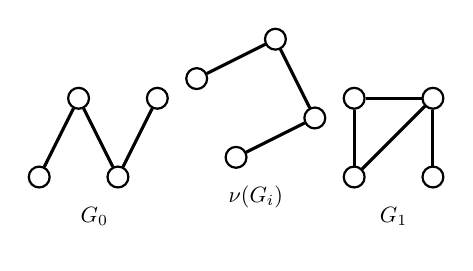
\begin{tikzpicture}[every node/.style={circle,thick,draw,scale=0.8}, line width=0.04cm]
    \node (A) at (0,-1.25) {};
    \node (B) at (1,-0.75) {};
    \node (C) at (-0.5,-0.25) {};
    \node (D) at (0.5,0.25) {};

    \draw (A) -- (B);
    \draw (B) -- (D);
    \draw (C) -- (D);

    \node[draw=none] (TEXT3) at (0.25,-1.75) {$\nu(G_i)$};

    \node (E) at (-1,-0.5) {};
    \node (F) at (-2,-0.5) {};
    \node (G) at (-2.5, -1.5) {};
    \node (H) at (-1.5, -1.5) {};

    \draw (G) -- (F);
    \draw (F) -- (H);
    \draw (H) -- (E);

    \node[draw=none] (TEXT) at (-1.8,-2) {$G_0$};

    \node (I) at (1.5, -0.5) {};
    \node (J) at (2.5,-0.5) {};
    \node (K) at (1.5,-1.5) {};
    \node (L) at (2.5,-1.5) {};

    \draw (I) -- (K);
    \draw (I) -- (J);
    \draw (K) -- (J);
    \draw (J) -- (L);

    \node[draw=none] (TEXT) at (2,-2) {$G_1$};
\end{tikzpicture}
\\
{\small Figure 1: Here the prover should answer with the index 0, since the graph $\nu(G_i)$ is isomorphic to $G_0$}
\end{center}

If the graphs are not isomorphic, and the prover always answers correctly, we will always be convinced, implying perfect completeness. On the other hand, if the graphs are isomorphic, the random graph $\nu(G_i)$ obtained is independent of the index $i$, and so for any answer the prover gives, there is a 50\% chance of being caught out, giving imperfect soundness.
\end{example}

If we forgive a margin of error, there is a magical result saying interactive proofs are efficient as can be.

\begin{theorem}[The PCP Theorem]
    For some $\varepsilon > 0$, every feasibly checkable theorem is checkable with imperfect soundness and imperfect completeness in only 3 questions!
\end{theorem}

Consider proving an integer has 1000 prime factors, or showing a graph is three colourable. The canonical proof of these claims (giving the prime decomposition, or giving the three colouring) is rather large. The PCP theorem claims that asking three random yes/no questions suffices to determine if the integer has exactly 1000 prime factors, and that the three coloring is precisely correct!

\begin{center}
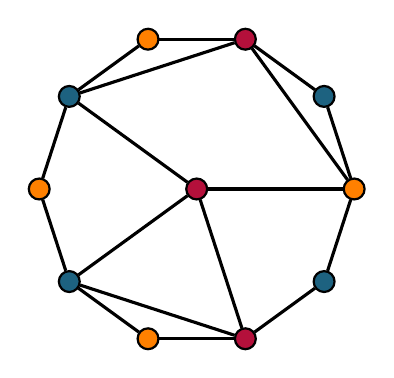
\begin{tikzpicture}[every node/.style={circle,thick,draw,scale=0.8}, line width=0.04cm]
    \node[fill = {rgb:red,255;green,22;blue,84}] (K) at (0:0) {};

    \node[fill = orange] (E) at (0:2) {};
    \node[fill = {rgb:red,36;green,123;blue,160}] (J) at (36:2) {};
    \node[fill = {rgb:red,255;green,22;blue,84}] (A) at (72:2) {};
    \node[fill = orange] (F) at (108:2) {};
    \node[fill = {rgb:red,36;green,123;blue,160}] (B) at (144:2) {};
    \node[fill = orange] (G) at (180:2) {};
    \node[fill = {rgb:red,36;green,123;blue,160}] (C) at (216:2) {};
    \node[fill = orange] (H) at (252:2) {};
    \node[fill = {rgb:red,255;green,22;blue,84}] (D) at (288:2) {};
    \node[fill = {rgb:red,36;green,123;blue,160}] (I) at (324:2) {};

    \draw (A) -- (B);
    \draw (A) -- (F);
    \draw (F) -- (B);
    \draw (B) -- (G);
%    \draw (B) -- (C);
    \draw (G) -- (C);
    \draw (C) -- (H);
    \draw (C) -- (D);
    \draw (H) -- (D);
    \draw (D) -- (I);
%    \draw (D) -- (E);
    \draw (I) -- (E);
    \draw (E) -- (A);
    \draw (E) -- (J);
    \draw (J) -- (A);
%    \draw (K) -- (A);
    \draw (K) -- (B);
    \draw (K) -- (C);
    \draw (K) -- (D);
    \draw (K) -- (E);
\end{tikzpicture}
\\
{\small Figure 2: A three coloring can fail at a single edge, like in the graph above. But what {\it three} questions prove a coloring is universally correct?}
\end{center}

 One way to think of this is that the PCP theorem says most {\it local} errors can be globalized. A graph can fail to be three colourable at a single edge, so we would have to check all edges to determine if a graph has been correctly three coloured. Similarily, a proof can have a single, localized mistake, which causes the entire proof to fail. The PCP theorem says that we can encode the graph and its colouring, or the proof of a theorem, as a randomized set of questions, such that any three questions chosen have a large chance of showing any errors -- local errors have been encoded globally!

Irit Dinur gave a good analogy of this globalization process. Imagine trying to determine if a slice of toast has jam on it, purely by tasting three bite sized pieces of the toast. With only a `localized' amount of jam, three random bites are unlikely to taste the jam. The encoding process of the PCP theorem can be compared to taking a knife, and smothering it over the piece of toast. If there is any jam on the bread, then the knife smothers jam all over the bread, and so a single bite will be able to determine if there was any jam on the bread to begin with.

\begin{center}
\includegraphics[scale=0.15]{JamOnToast.png}
\\
{\small Figure 3: It only takes one or two bites to determine if there is jam on the bread after it has been spread.}
\end{center}

The PCP theorem is a remarkable fact, but its ideas have yet to gestate outside the field of complexity theory it was invented in. It says that languages provide a way to efficiently encode {\it local} properties of mathematical objects {\it globally}, where they can be easily checked. I wrote this article because I'm sure there's another corner of mathematics where jam spreading can come in handy!

\begin{thebibliography}{9}

\bibitem{aroraBarak}
Sanjeev Arora, Boaz Barak. 2009.
``Computational Complexity: A Modern Approach'' {\it Cambridge University Press}.

\bibitem{odonell}
Ryan O'Donnell. 2012.
``Analysis of Boolean Functions'' {\it Cambridge University Press}. Available at: \url{http://www.contrib.andrew.cmu.edu/~ryanod/}

\bibitem{dinur}
Irit Dinur. 2011.
``PCPs and Expander Graphs'' {\it Microsoft Research Talks}. Available at: \url{https://www.microsoft.com/en-us/research/video/pcps-and-expander-graphs/}

\end{thebibliography}

\end{multicols}

\end{document}